\documentclass{ifacconf}

\usepackage{natbib}            % you should have natbib.sty
\usepackage[utf8]{inputenc}    % Eingabe von Umlauten im Editor, dieser sollte dann auch auf utf8 Encoding eingestellt sein
\usepackage{graphicx}          % Include this line if your 
                               % document contains figures,
%\usepackage[dvips]{epsfig}    % or this line, depending on which
                               % you prefer.
                               
\usepackage{units}

% for German
% \usepackage{ngerman}           % neue Deutsche Rechtschreibung, Silbentrennung
% \usepackage[T1]{fontenc}       % Trennung mit Umlauten

% to include tikz pictures of figure created with matlab2tikz, see also file ``plotFigureTest.m''
\usepackage{tikz}
\usepackage{pgfplots}
\pgfplotsset{compat=newest}  % use newest version of pgfplots
\usepackage{amsmath}  % useful for math

% to include the legend into the caption. The commands are
%\mlLineLegend{red}
%\mlLineLegendDashed{red}
%\mlLineLegendDotted{red}
%\mlLineLegendDashDotted{red}
%\mlPointLegend{red}
\newlength{\mlLegendThickness}
\setlength{\mlLegendThickness}{0.4mm}
\newlength{\mlLegendHeight}
\setlength{\mlLegendHeight}{0.6ex}
\newcommand{\mlLineLegend}[1]{\mbox{\color{#1}
\protect\rule[\mlLegendHeight]{3mm}{\mlLegendThickness}\hspace*{-1mm}
}}
\newcommand{\mlLineLegendDashed}[1]{\mbox{\color{#1}
\protect\rule[\mlLegendHeight]{1.5mm}{\mlLegendThickness}\hspace*{0mm}
\protect\rule[\mlLegendHeight]{1.5mm}{\mlLegendThickness}\hspace*{-1mm}
}}
\newcommand{\mlLineLegendDotted}[1]{\mbox{\color{#1}
\protect\rule[\mlLegendHeight]{0.4mm}{\mlLegendThickness}\hspace*{0mm}
\protect\rule[\mlLegendHeight]{0.4mm}{\mlLegendThickness}\hspace*{0mm}
\protect\rule[\mlLegendHeight]{0.4mm}{\mlLegendThickness}\hspace*{0mm}
\protect\rule[\mlLegendHeight]{0.4mm}{\mlLegendThickness}\hspace*{-1mm}
}}
\newcommand{\mlLineLegendDashDotted}[1]{\mbox{\color{#1}
\protect\rule[\mlLegendHeight]{1.5mm}{\mlLegendThickness}\hspace*{0mm}
\protect\rule[\mlLegendHeight]{0.4mm}{\mlLegendThickness}\hspace*{0mm}
\protect\rule[\mlLegendHeight]{1.5mm}{\mlLegendThickness}\hspace*{0mm}
\protect\rule[\mlLegendHeight]{0.4mm}{\mlLegendThickness}\hspace*{-1mm}
}}
\newcommand{\mlPointLegend}[1]{\mbox{\color{#1}
\protect\rule[\mlLegendHeight]{0.4mm}{\mlLegendThickness}\hspace*{-0.75mm}
}}

\begin{document}

\begin{frontmatter}
	
\title{Gruppe B-Mo2: \\ Abschlussprotokoll}
% include all authors, underline corresponding author
\author{\underline{Yuchan Bian},} 
\author{Jiaqi Qin,}
\author{E. Boateng} 


\begin{abstract}                          % Abstract of not more than 250 words.

\end{abstract}

\end{frontmatter}

\section{Regler}
\subsection{Reglerauswahl}
Durch die Aufgabenstellung der Trajektorien leiten sich die Zielvorgaben des Reglerentwurfs ab. Der Helikopter soll nicht nur stabilisiert werden sondern einer Trajektorienvorgabe möglichst robust und ohne Sollwertabweichung folgen. Zur Erfüllung der Aufgabenstellung werden an den Regler folgende Anforderung gestellt:
\begin{itemize}
	\item Der geschlossene Kreis soll stabil sein.
	\item  Die bleibende Regelabweichung von $\alpha$ und $\beta$  soll so gering sein, dass der Helikopter entlang einer vorgegebenen Trajektorie fliegen kann.
	\item Der Helikopter kann die vorgegebene Position schnell erreichen.
\end{itemize}
Ein LQR-Regler vereint diese Eigenschaften. Erweitert um einen I-Anteil, der eine Sollwertabweichung der Trajektorie minimiert, ist hier ein Ansatz zu einem LQI-Regelrentwurf beschrieben. Deshalb haben wir einen LQI-Regler ausgewählt.

\subsection{Linearisierung}
Der Zustandsvektor x, die Schubkraft der Rotoren als Eingangsvektor u und der Ausgang y lauten wie folgend:
\begin{equation}
	x=\left[\begin{array}{c}
		\alpha,\beta,\gamma,\dot{\alpha},\dot{\beta},\dot{\gamma}\
	\end{array}\right]^T
\end{equation}
\begin{equation}
	u=\left[\begin{array}{c}
		F_{f}\\F_{b}
	\end{array}\right]
\end{equation}
\begin{equation}
	y=\left[\begin{array}{c}
		\alpha\\\beta\\\gamma
	\end{array}\right]
\end{equation}
Um das System leichter zu analysieren und die Basis fuer eine spaetere Regelerauslegung zu generieren, wird das System um eine Ruhelage linearisiert. Als Linearisierungspunkt wird
\begin{equation}
	\bar{x} =\left[\begin{array}{c}
		0,-3^{\circ},0,0,0,0
	\end{array}\right] ^{T}
\end{equation}
gewaehlt.
Auf Basis des Arbeitspunktes wird die Schubkraft als Eingang fuer die Ruhelage bestimmt. 
\begin{equation}
	\bar{u}=\left[\begin{array}{c}
		0.5873\\0.5873
	\end{array}\right]
\end{equation}

Für die Systemmatrix A ergibt sich durch Ableiten nach dem Zustandsvektor x und einsetzen des Linearisierungspunktes:
\begin{equation}
	A=\left[\begin{array}{llllll}
		0 & 0 & 0 & 1 & 0 & 0 \\
		0 & 0 & 0 & 0 & 1 & 0 \\
		0 & 0 & 0 & 0 & 0 & 1 \\
		0 & 0 & -0.6921& 0 & 0 & 0 \\
		0 & -0.0359& 0 & 0 & 0 & 0 \\
		0 & 0 & 0 & 0 & 0 & 0
	\end{array}\right]
\end{equation}
Die Eingangsmatrix B ergibt sich durch Jacobi-Matrix abgeleitet nach den Eingangsgrößen und einsetzen des Linearisierungspunktes zu:
\begin{equation}
	B=\left[\begin{array}{cc}
		0 & 0 \\
		0 & 0 \\
		0 & 0 \\
		0 & 0 \\
		0.5832 & 0.5832\\
		5.5383& -5.5383\\
	\end{array}\right]
\end{equation}
Die Ausgangsmatrix C ergibt sich zu
\begin{equation}
	\begin{array}{l}
		C=\left[\begin{array}{llllll}
			1 & 0 & 0 & 0 & 0 & 0 \\
			0 & 1 & 0 & 0 & 0 & 0 \\
			0 & 0 & 1 & 0 & 0 & 0
		\end{array}\right] 
	\end{array}
\end{equation}

Die Durchgriffsmatrix D ergibt sich zu Null und ist mit folgender Dimension durch 
\begin{equation}
	\begin{array}{l}
		D=\left[\begin{array}{ll}
			0 & 0 \\
			0 & 0 \\
			0 & 0
		\end{array}\right]
	\end{array}
\end{equation}
gegeben.\\

Bei weiteren Untersuchungen eines Beobachters und der Regelerauslegung ist darauf zu achten, dass das linearisierte Modell nun mit den Abweichungen $\Delta{x}$, $\Delta{u}$, $\Delta{y}$ der Größen arbeitet. 
 \begin{equation}{}
 	\Delta{x}=x-\bar{x},
 	\Delta{u}=u-\bar{u},
 	\Delta{y}=y-\bar{y}
 \end{equation}
Das linearisierte System ist vollständig gegeben durch:
\begin{equation}{}
	 \Delta{\dot{x}}=A \Delta{x}+B \Delta{u}  \qquad \Delta{y}=C\Delta{x}+ D \Delta{u} 
\end{equation}
mit der Anfangsbedingung 
 \begin{equation}{}
	\Delta{x}(0)=x(0)-\bar{x}
\end{equation}
\subsection{Steuerbarkeit und Beobachtbarkeit}
Die Steuerbarkeit und Beobachtbarkeit von Systemen sind in Matlab gerechnet und sie haben beiden vollen Rang. Das lineare System ist steuerbar und beobachtbar.

\subsection{LQI-Regelstruktur}
Die Regelkreisstruktur des linearisierten Systems stellt sich wie folgend dar(Abbildung \ref{fig:Regelstruktur des linearisierten Systems}):\\
\begin{figure} [h]
	\begin{center} 
		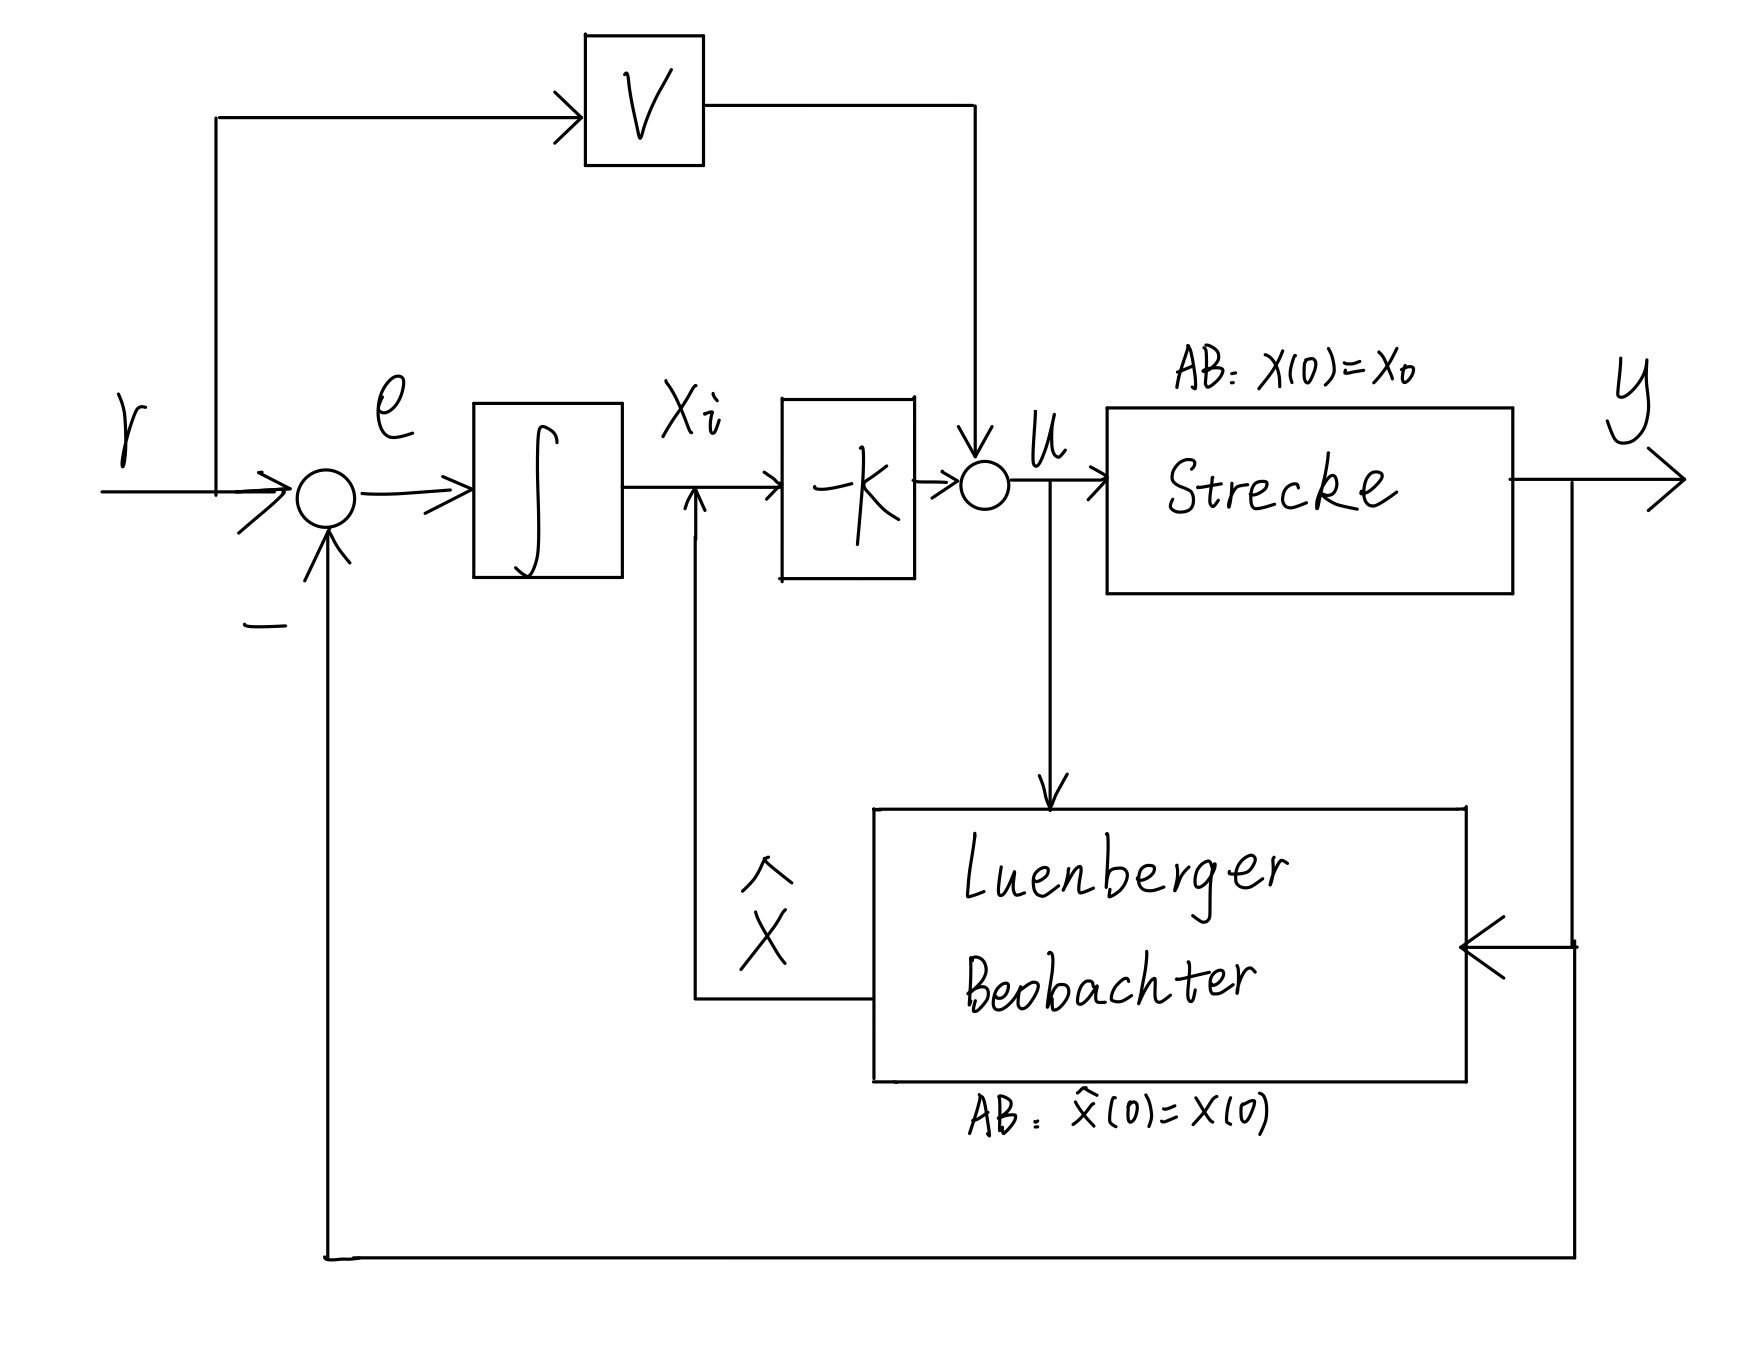
\includegraphics[scale=0.14]{Regelstruktur des linearisierten Systems} 
		\caption{Regelstruktur des linearisierten Systems}\label{fig:Regelstruktur des linearisierten Systems}
	\end{center}
\end{figure}\\
Die Reglerstruktur für das nichtlineare Modell und Black Box Modell stellt sich wie folgend dar(Abbildung \ref{fig:Reglerstruktur für das nichtlineare Modell und Black Box Modell}):\\
\begin{figure} [h]
	\begin{center} 
		\includegraphics[scale=0.18]{Reglerstruktur für das nichtlineare Modell und Black Box Modell} 
		\caption{Reglerstruktur für das nichtlineare Modell und Black Box Modell}\label{fig:Reglerstruktur für das nichtlineare Modell und Black Box Modell}
	\end{center}
\end{figure}\\


Der LQI Regler wird mittels Matlab Befehl "lqi" angewendet. Für eine Strecke mit den Zustandsraumgleichungen:
 \begin{equation}{}
\begin{split}
	\left[\begin{array}{l}
		\Delta \dot{x} \\
		\Delta \dot{x}_{i}
	\end{array}
\right] =&\left[\begin{array}{c}
		A \Delta x+B \Delta u \\
		\Delta r-\Delta y
	\end{array}\right] \\
=&\underbrace{\left[\begin{array}{cc}
			A & 0 \\
			-C_{neu} & 0
		\end{array}\right]}_{A_{LQI}}\left[\begin{array}{c}
		\Delta x \\
		\Delta x_{i}
	\end{array}\right]+\underbrace{\left[\begin{array}{c}
			B \\
			0
		\end{array}\right]}_{B_{LQI}} \Delta u+\left[\begin{array}{c}
		0 \\
		I
	\end{array}\right] \Delta r
\end{split}
\end{equation}
$\Delta{x} \in R^{6\times1}$ und $\Delta{x_{i}}$ ist der Integratorausgang für Fehler e $\in R^{2\times1}$. \\
\begin{equation}
\Delta{y}_{neu}=C_{neu}\Delta{x}
\end{equation}
\begin{equation}
	y_{neu}=\left[\begin{array}{c}
		\alpha\\\beta
	\end{array}\right]
\end{equation}
Die neue Matrix $A_{LQI}$ in jetztigen System lautet:
\begin{equation}
	A_{LQI}=\left[\begin{array}{llllllll}
		0 & 0 & 0 & 1 & 0 & 0 & 0 &0 \\
		0 & 0 & 0 & 0 & 1 & 0 & 0 &0 \\
			0 & 0 & 0 & 0 & 0 & 1 & 0 &0 \\
		0 & 0 & -0.6921 & 0 & 0 & 0 & 0 &0 \\
		0 & -0.0359 & 0 & 0 & 0 & 0 & 0 &0 \\
			0 & 0 & 0 & 0& 0 & 0 & 0 &0 \\
				-1 & 0 & 0 & 0 & 0 & 0 & 0 &0 \\
					0 & -1 & 0 & 0& 0 & 0 & 0 &0 
	\end{array}\right]
\end{equation}
Die Eingangsmatrix $B_{LQI} $:
\begin{equation}
	B_{LQI} =\left[\begin{array}{cc}
		0 & 0 \\
		0 & 0 \\
		0 & 0 \\
		0 & 0 \\
		0.5832& 0.5832\\
		5.5383& -5.5383\\
		0 & 0 \\
		0 & 0 
	\end{array}\right]
\end{equation}

Die neue Ausgangsmatrix $C_{neu}$ ergibt sich zu
\begin{equation}
	\begin{array}{l}
		C_{neu}=\left[\begin{array}{llllll}
			1 & 0 & 0 & 0 & 0 & 0 \\
			0 & 1 & 0 & 0 & 0 & 0 \\
		\end{array}\right] 
	\end{array}
\end{equation}

Die Matrix $D_{neu}$ lautet:
\begin{equation}
	\begin{array}{l}
		D_{neu}=\left[\begin{array}{ll}
			0 & 0 \\
			0 & 0 
		\end{array}\right]
	\end{array}
\end{equation}


Denn wir brauchen nur die $\alpha$ und $\beta$ für Trajektorie, das bedeutet, 
\begin{equation}
	r=\left[\begin{array}{c}
		\alpha_{r}\\\beta_{r}
	\end{array}\right]
\end{equation}

Die Zustandsrückfüheung hat die Form
\begin{equation}{}
	\Delta{u} = -K _{LQI}[\Delta{x}; \Delta {x_{i}}]
\end{equation}
%\begin{equation}
	%x=\left[\begin{array}{c}
	%	\alpha\\\beta\\\gamma\\\dot{\alpha}\\\dot{\beta}\\\dot{\gamma}\ 
	%\end{array}\right] 	
%\end{equation}
Und $K _{LQI}\in R^{2\times8}$.\\

Das resultierende Gain $K _{LQI}(K _{LQR},K _{I})$ ist:\\
\begin{equation}
	\begin{array}{l}
		K_{LQR}=\left[\begin{array}{llllll}
				-17.9241& 8.3305& 6.2126& -17.4933 & 4.0967& 1.2735\\
			17.9241& 8.3305& -6.2126& 17.4933&  4.0967&-1.2735 
		\end{array}\right] 
	\end{array}
\end{equation}

\begin{equation}
	\begin{array}{l}
		K _{I}=\left[\begin{array}{ll}
			6.3246& -3.1623\\
			-6.3246 &-3.1623
		\end{array}\right]
	\end{array}
\end{equation}

Und der Vorfilter $V= -(C_{neu}(A-BK_{LQR})^{-1}B)^{-1} $ ist:
\begin{equation}
	\begin{array}{l}
		V=\left[\begin{array}{ll}
			-17.9241& 8.3613\\
			17.9241 &8.3613
		\end{array}\right]
	\end{array}
\end{equation}

Die Eigenwerte des geschlossenen Regelkreises ergeben sich zu:
\begin{equation}
	EW=\left[\begin{array}{c}
		-7.7685\\
		-0.4861+0.7260i\\
		-0.4861-0.7260i\\
		-0.9196+0.2243i\\
		-0.9196-0.2243i\\
		-0.6375+0.7327i\\
		-0.6375-0.7327i\\
	   -0.8754
	\end{array}\right]
\end{equation}
Die negativen Realteile der Eigenwerte zeigen alles asympotisch stabiles Verhalten des geschlossenen Regelkreises.

Der LQI-Regler wird durch Matlab-Befehl ''lqi'' angewandet. Dieses Steuergesetz stellt sicher, dass die Ausgabe y die Referenztrajektorie r gut trackt. Bei MIMO-Systemen entspricht die Anzahl der Integratoren der Dimension der Ausgabe y. [K, S, e] = lqi (SYS, Q, R, N) berechnet die optimale Verstärkungsmatrix K unter Berücksichtigung eines Zustandsraummodells SYS für die Matrizen Q, R, N (In unseren System wählen wir N=0). u und y sind absolute Werte für das linearisiertes Modell. Aber $\Delta u$ und $\Delta y$ sollen für das nichtlinearisiertes Modell angewendet werden.

\begin{equation}
Q=\left[\begin{array}{llllllll}
	200& 0 & 0 & 0 & 0 & 0 & 0 & 0\\
	0 & 88 & 0 & 0 & 0 & 0 & 0 & 0\\
	0 & 0 & 20& 0& 0 & 0 & 0 & 0\\
    0 & 0 & 0 & 15 & 0 & 0 & 0 & 0\\
    0 & 0 & 0 & 0 & 5 & 0 & 0 & 0\\
    0 & 0 & 0 & 0 & 0 & 1 & 0 & 0\\
    0 & 0 & 0 & 0 & 0 & 0 & 80& 0\\
	0 & 0 & 0 & 0 & 0 & 0 & 0 & 20
\end{array}\right]
\end{equation}
\begin{equation}
	\begin{array}{l}
		R=\left[\begin{array}{ll}
			1 & 0 \\
			0 & 1 
		\end{array}\right]
	\end{array}
\end{equation}

\subsection{Beobachterentwurf}
Da die Winkelgeschwindigkeiten des Helikopters nicht messbar sind, ist ein Beobachter erforderlich, welcher diese fehlenden Zustände schätzt. Der Luenberger Beobachter wird angewendet, um die Zustände zu rekonstruieren. Die Pole des Beobachters wurden nach diese Befehl: $p = min(real(EW))\times3$ ausgewählt. Die Pole p in unseren System lautet:
\begin{equation}
	p =\left[\begin{array}{c}
		-23,-23.1,-23.2,-23.3,-23.4,-23.5
	\end{array}\right] ^{T}
\end{equation}
Und das resultierende Gain L vom Beobachter ist:
\begin{equation}
	L=\left[\begin{array}{lll}
		46.9000& 0 & 0 \\
		0 & 46.3000& 0 \\
		0 & 0 & 46.3000\\
		549.9000 & 0 & -0.6921 \\
		0 & 535.8841 & 0 \\
		0 & 0 & 535.9000\\
	\end{array}\right]
\end{equation}


%\bibliographystyle{alpha}        % Include this if you use bibtex 
%\bibliography{autosam}           % and a bib file to produce the 
%\bibliography{autosam}
                                 % bibliography (preferred). The
                                 % correct style is generated by
                                 % Elsevier at the time of printing.

\begin{thebibliography}{1}
	
\bibitem{handbook}Handbook Control of a 3-DOF Helicopter
\\ IST, University of Stuttgart, Germany
\\ Corona Edition Winter term 2020/21
	
\bibitem{Regelkreisstrukturen}Regelkreisstrukturen
\\ IST, University of Stuttgart, Germany	

	
	
	
\end{thebibliography}

%\appendix
\end{document}